\documentclass[12pt,a4paper]{article}

% ─── Page Layout ───────────────────────────────────────────────────────────────
\usepackage[a4paper, margin=0.8in, headheight=14pt]{geometry}

% ─── Fonts (XeLaTeX) ───────────────────────────────────────────────────────────
\usepackage{fontspec}
\usepackage{unicode-math}
\setmainfont{TeX Gyre Pagella}
\setmonofont[Scale=0.88]{TeX Gyre Cursor}
\setmathfont{Latin Modern Math}

% ─── Packages ──────────────────────────────────────────────────────────────────
\usepackage{xcolor}
\usepackage{colortbl}
\usepackage{titlesec}
\usepackage{enumitem}
\usepackage{tabularx}
\usepackage{booktabs}
\usepackage{array}
\usepackage{amsmath}
\usepackage{tikz}
\usetikzlibrary{shapes.geometric, arrows.meta, positioning, calc, fit, decorations.pathreplacing}
\usepackage{tcolorbox}
\tcbuselibrary{skins, breakable}
\usepackage{hyperref}
\usepackage{fancyhdr}
\usepackage{graphicx}
\usepackage{microtype}
\hyphenpenalty=10000
\exhyphenpenalty=10000
\sloppy
\usepackage{caption}
\usepackage{setspace}
\usepackage{multirow}
\usepackage{tocloft}

% ─── Q&A helper ────────────────────────────────────────────────────────────────
\newcommand{\Q}[1]{\textbf{#1}\par\noindent\ignorespaces}

% ─── Colour Palette ────────────────────────────────────────────────────────────
\definecolor{myred}{RGB}{196,30,58}
\definecolor{mydark}{RGB}{30,30,50}
\definecolor{mygreen}{RGB}{14,120,80}
\definecolor{myteal}{RGB}{0,130,140}
\definecolor{myamber}{RGB}{180,100,0}
\definecolor{mypurple}{RGB}{100,30,160}
\definecolor{mygray}{RGB}{246,247,249}
\definecolor{mgframe}{RGB}{180,185,200}
\definecolor{watermark}{RGB}{145,150,170}
\definecolor{hdrred}{RGB}{250,232,235}
\definecolor{hdrgreen}{RGB}{220,244,233}
\definecolor{hdrteal}{RGB}{220,242,244}
\definecolor{hdramber}{RGB}{253,242,215}
\definecolor{hdrpurple}{RGB}{238,228,255}
\definecolor{hdrgray}{RGB}{238,240,245}
\definecolor{rowalt}{RGB}{250,251,253}

% ─── Section Formatting ────────────────────────────────────────────────────────
\titleformat{\section}
  {\large\bfseries\color{myred}}{\thesection.}{0.5em}{}
  [\vspace{1pt}{\color{myred}\rule{\linewidth}{0.8pt}}]
\titleformat{\subsection}
  {\normalsize\bfseries\color{myteal}}{\thesubsection}{0.5em}{}
\titlespacing*{\section}{0pt}{18pt}{7pt}
\titlespacing*{\subsection}{0pt}{11pt}{4pt}

% ─── Paragraph ─────────────────────────────────────────────────────────────────
\setlength{\parindent}{0pt}
\setlength{\parskip}{4pt}

% ─── TOC Styling ───────────────────────────────────────────────────────────────
\renewcommand{\cfttoctitlefont}{\large\bfseries\color{myred}}
\renewcommand{\cftaftertoctitle}{\par\noindent{\color{myred}\rule{\linewidth}{0.8pt}}}
\setlength{\cftbeforetoctitleskip}{0pt}
\setlength{\cftaftertoctitleskip}{6pt}
\renewcommand{\cftsecfont}{\normalsize\bfseries\color{mydark}}
\renewcommand{\cftsecpagefont}{\normalsize\bfseries\color{mydark}}
\renewcommand{\cftsecleader}{\cftdotfill{\cftdotsep}}
\setlength{\cftbeforesecskip}{7pt}
\renewcommand{\cftsubsecfont}{\small\color{mydark}}
\renewcommand{\cftsubsecpagefont}{\small\color{mydark}}
\setlength{\cftbeforesubsecskip}{3pt}
\setlength{\cftsubsecindent}{1.4em}

% ─── Table helpers ─────────────────────────────────────────────────────────────
\renewcommand{\arraystretch}{1.45}
\setlength{\tabcolsep}{6pt}
\arrayrulecolor{mydark}
\newcolumntype{B}[1]{>{\small\bfseries\raggedright\arraybackslash}m{#1}}
\newcolumntype{Y}{>{\small\raggedright\arraybackslash}X}
\renewcommand{\tabularxcolumn}[1]{m{#1}}

% ─── Header / Footer ───────────────────────────────────────────────────────────
\pagestyle{fancy}
\fancyhf{}
\fancyhead[L]{\small\color{myred}\textbf{OE-EC604A}\;\color{mydark}--- Electronic Measurement \& Instruments}
\fancyhead[R]{\small\color{myteal}\textbf{Module 4 Notes}}
\fancyfoot[C]{\small\color{mydark}\thepage}
\fancyfoot[R]{\small\color{watermark}\textit{\copyright\ Biraj}}
\renewcommand{\headrulewidth}{0.5pt}
\renewcommand{\footrulewidth}{0.3pt}

% ─── Hyperref ──────────────────────────────────────────────────────────────────
\hypersetup{
  colorlinks=true, linkcolor=myteal, urlcolor=myteal,
  pdfauthor={Biraj Sarkar},
  pdftitle={OE-EC604A --- Module 4 Notes}
}

% ─── tcolorbox styles ──────────────────────────────────────────────────────────
\tcbset{
  tikzbox/.style={
    colback=mygray, colframe=mgframe, boxrule=0.6pt, arc=4pt,
    left=8pt, right=8pt, top=6pt, bottom=6pt,
    colbacktitle=mgframe, coltitle=mydark,
    fonttitle=\small\bfseries
  },
  defbox/.style={
    colback=hdrgreen, colframe=mygreen, boxrule=0.8pt, arc=4pt,
    left=9pt, right=9pt, top=6pt, bottom=6pt,
    colbacktitle=mygreen, coltitle=white,
    fonttitle=\small\bfseries
  },
  formulabox/.style={
    colback=hdrteal, colframe=myteal, boxrule=0.8pt, arc=4pt,
    left=9pt, right=9pt, top=7pt, bottom=7pt,
    colbacktitle=myteal, coltitle=white,
    fonttitle=\small\bfseries
  },
  examplebox/.style={
    colback=hdramber, colframe=myamber, boxrule=0.8pt, arc=4pt,
    left=9pt, right=9pt, top=6pt, bottom=6pt,
    colbacktitle=myamber, coltitle=white,
    fonttitle=\small\bfseries
  },
  masonbox/.style={
    colback=hdrpurple, colframe=mypurple, boxrule=0.8pt, arc=4pt,
    left=9pt, right=9pt, top=6pt, bottom=6pt,
    colbacktitle=mypurple, coltitle=white,
    fonttitle=\small\bfseries
  },
  exambox/.style={
    colback=hdrpurple, colframe=mypurple, boxrule=1pt, arc=5pt,
    left=10pt, right=10pt, top=8pt, bottom=8pt,
    colbacktitle=mypurple, coltitle=white,
    fonttitle=\bfseries,
    breakable, title after break={\textbf{Frequently Asked / Viva Questions (contd.)}}}
}
% Make all boxes breakable across pages
\tcbset{breakable}

% ─── TikZ styles ───────────────────────────────────────────────────────────────
\tikzset{
  block/.style={rectangle, draw=myteal, fill=hdrteal,
    text width=2.4cm, align=center, minimum height=0.95cm,
    font=\small, rounded corners=3pt, line width=0.7pt},
  redblock/.style={rectangle, draw=myred, fill=hdrred,
    text width=2.4cm, align=center, minimum height=0.95cm,
    font=\small, rounded corners=3pt, line width=0.7pt},
  greenblock/.style={rectangle, draw=mygreen, fill=hdrgreen,
    text width=2.4cm, align=center, minimum height=0.95cm,
    font=\small, rounded corners=3pt, line width=0.7pt},
  amberblock/.style={rectangle, draw=myamber, fill=hdramber,
    text width=2.4cm, align=center, minimum height=0.95cm,
    font=\small, rounded corners=3pt, line width=0.7pt},
  purpblock/.style={rectangle, draw=mypurple, fill=hdrpurple,
    text width=2.4cm, align=center, minimum height=0.95cm,
    font=\small, rounded corners=3pt, line width=0.7pt},
  sumjunc/.style={circle, draw=myamber, fill=hdramber,
    minimum size=0.62cm, font=\small, line width=0.8pt},
  arrow/.style={-Stealth, thick, color=mydark},
  redarrow/.style={-Stealth, thick, color=myred},
  line/.style={thick, color=mydark}
}

% ═══════════════════════════════════════════════════════════════════════════════
\begin{document}
% ═══════════════════════════════════════════════════════════════════════════════

\begin{center}
  {\LARGE\bfseries\color{myred} OE-EC604A --- Electronic Measurement \& Measuring Instruments}\\[5pt]
  {\normalsize\color{mydark} Semester VI \quad$\bullet$\quad 3L:0T:0P \quad$\bullet$\quad 3 Credits}\\[3pt]
  {\normalsize\color{myteal}\textbf{Module 4 Exam Notes: Transducers}}\\[3pt]
  {\small\color{mydark} CGEC \;$|$\; B.Tech ECE (2023--27) \;$|$\; \textit{Biraj Sarkar}}
\end{center}
\vspace{2pt}
\noindent{\color{myred}\rule{\linewidth}{1.5pt}}
\vspace{2pt}

\hypersetup{linkcolor=mydark}
\tableofcontents
\hypersetup{linkcolor=myteal}
\newpage

% ===============================================================================
\section{Introduction \& Classification}
% ===============================================================================

A \textbf{Transducer} is a physical device that converts energy from one form into another, typically transforming a physical parameter (measurand) into a proportional electrical signal.

\subsection{Key Classifications}
\begin{itemize}[leftmargin=*, itemsep=3.5pt]
  \item \textbf{Active vs. Passive Transducers:}
    - \textbf{Active (Self-generating):} Generates its own electrical output without requiring an external power source (e.g., Piezoelectric crystal, Thermocouple, Solar cell).
    - \textbf{Passive:} Requires an external excitation voltage source to function, modulating its resistance, capacitance, or inductance (e.g., Strain gauge, LVDT, Thermistor, RTD).
  \item \textbf{Primary vs. Secondary Transducers:}
    - \textbf{Primary:} Interacts directly with the measurand, converting it to a mechanical displacement (e.g., Bourdon tube).
    - \textbf{Secondary:} Converts the output of the primary transducer into an electrical signal (e.g., LVDT connected to Bourdon tube).
  \item \textbf{Analog vs. Digital Transducers:}
    - \textbf{Analog:} Outputs a continuous amplitude voltage signal (e.g., Thermocouple).
    - \textbf{Digital:} Outputs discrete pulse trains or binary codes (e.g., Shaft encoder).
\end{itemize}

% ===============================================================================
\section{Strain Gauges \& Temperature Transducers}
% ===============================================================================

\subsection{Strain Gauges \& Gauge Factor Derivation}
A strain gauge measures mechanical strain based on the piezoresistive effect: when a wire is stretched, its resistance changes due to change in length, cross-sectional area, and resistivity.

\begin{tcolorbox}[formulabox, title={\textbf{Gauge Factor (G) Derivation}}]
Resistance of a wire is $R = \rho \cdot \frac{L}{A}$. Taking the natural log on both sides:
$$\ln R = \ln \rho + \ln L - \ln A$$
Differentiating with respect to strain $\epsilon$:
$$\frac{dR}{R} = \frac{d\rho}{\rho} + \frac{dL}{L} - \frac{dA}{A}$$
Since area $A = \frac{\pi D^2}{4} \implies \ln A = \ln(\pi/4) + 2\ln D \implies \frac{dA}{A} = 2\frac{dD}{D}$. Thus:
$$\frac{dR}{R} = \frac{dL}{L} - 2\frac{dD}{D} + \frac{d\rho}{\rho}$$
Poisson's ratio is defined as $\nu = -\frac{dD/D}{dL/L} \implies \frac{dD}{D} = -\nu \frac{dL}{L}$. Substituting this:
$$\frac{dR}{R} = \frac{dL}{L} + 2\nu\frac{dL}{L} + \frac{d\rho}{\rho} = \frac{dL}{L}(1 + 2\nu) + \frac{d\rho}{\rho}$$
Dividing both sides by longitudinal strain $\epsilon = dL/L$:
$$G = \frac{dR/R}{dL/L} = 1 + 2\nu + \frac{d\rho/\rho}{dL/L}$$
where:
- $1$: Resistance change due to length change.
- $2\nu$: Resistance change due to area change.
- $\frac{d\rho/\rho}{dL/L}$: Piezoresistive effect (resistivity change). For metals, $G \approx 2.0$.
\end{tcolorbox}

\subsection{Temperature Transducers}
\begin{itemize}[leftmargin=*, itemsep=3.5pt]
  \item \textbf{RTD (Resistance Temperature Detector):} Made of pure metals (Platinum/Nickel). Positive temperature coefficient (PTC) $\implies$ resistance increases linearly with temperature: $R_T = R_0(1 + \alpha T)$. Stable, highly accurate.
  \item \textbf{Thermistor:} Made of semiconductor oxides. High negative temperature coefficient (NTC) $\implies$ resistance decreases exponentially with temperature. Extremely sensitive but non-linear.
  \item \textbf{Thermocouple:} Active transducer based on the Seebeck effect: when two dissimilar metals are joined at two junctions held at different temperatures, an electromotive force (EMF) is generated ($E = aT + bT^2$). Self-powered, wide temperature range.
\end{itemize}

% ===============================================================================
\section{LVDT \& Other Special Transducers}
% ===============================================================================

\subsection{LVDT (Linear Variable Differential Transformer)}
An \textbf{LVDT} is a passive inductive transducer used to measure linear displacement.
- \textbf{Structure:} Consists of a single primary winding (excited by AC), two secondary windings ($S_1$ and $S_2$) wound symmetrically on a hollow cylinder, and a movable soft iron core inside.
- \textbf{Working:} Secondary windings are connected in \textbf{series opposition}, so the output voltage is $E_o = E_{s1} - E_{s2}$.
  - At \textbf{Null Position} (core exactly centered): Magnetic coupling to both secondaries is identical $\implies E_{s1} = E_{s2} \implies E_o = 0\,\text{V}$.
  - Displacement to \textbf{Left}: Coupling to $S_1$ increases $\implies E_{s1} > E_{s2} \implies E_o$ is in-phase with input.
  - Displacement to \textbf{Right}: Coupling to $S_2$ increases $\implies E_{s2} > E_{s1} \implies E_o$ is out-of-phase by $180^\circ$.

\begin{tcolorbox}[tikzbox, title={LVDT Circuit Diagram}]
\centering
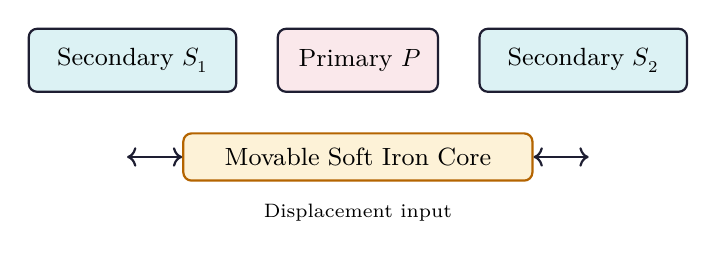
\begin{tikzpicture}[node distance=0.4cm and 0.5cm, thick, font=\small]
  % Define local node styles
  \tikzset{
    secblock/.style={rectangle, draw=mydark, fill=hdrteal, text width=2.4cm, align=center, minimum height=0.8cm, rounded corners=3pt},
    priblock/.style={rectangle, draw=mydark, fill=hdrred, text width=1.8cm, align=center, minimum height=0.8cm, rounded corners=3pt},
    coreblock/.style={rectangle, draw=myamber, fill=hdramber, text width=4.2cm, align=center, minimum height=0.6cm, rounded corners=3pt}
  }
  
  % Place Coils
  \node[secblock] (s1) {Secondary $S_1$};
  \node[priblock, right=of s1] (p) {Primary $P$};
  \node[secblock, right=of p] (s2) {Secondary $S_2$};
  
  % Place Core
  \node[coreblock, below=0.5cm of p] (core) {Movable Soft Iron Core};
  
  % Draw displacement arrows
  \draw[arrow, <->] ($(core.west) - (0.7, 0)$) -- (core.west);
  \draw[arrow, <->] (core.east) -- ($(core.east) + (0.7, 0)$);
  
  \node[below=0.15cm of core, font=\scriptsize] {Displacement input};
\end{tikzpicture}
\end{tcolorbox}

\subsection{Piezoelectric Transducer}
- \textbf{Principle:} Active transducer based on the piezoelectric effect. When mechanical force $F$ is applied to asymmetrical crystals (Quartz, Rochelle salt), electric charges $Q$ are generated on opposite faces: $Q = d \cdot F$, where $d$ is charge sensitivity. Output voltage is $V_o = g \cdot t \cdot P$ (where $g$ = voltage sensitivity, $t$ = thickness, $P$ = pressure).
- Used for dynamic force/pressure/vibration measurements. Cannot measure static displacement.

\newpage
% ===============================================================================
% MANDATORY QUICK REVISION PAGE
% ===============================================================================
\begin{center}
  {\large\bfseries\color{myred} Quick Revision --- Module 4}\\[3pt]
  {\small\color{mydark} Transducers $|$ OE-EC604A}
\end{center}
\noindent{\color{myred}\rule{\linewidth}{1.2pt}}
\vspace{4pt}

\begin{tcolorbox}[formulabox, title={\textbf{Key Transducer Formulas}}]
$$\text{Strain Gauge factor:} \quad G = 1 + 2\nu + \frac{d\rho/\rho}{d\epsilon} \qquad \frac{dR}{R} = G \cdot \epsilon$$
$$\text{RTD resistance:} \quad R_T = R_0(1 + \alpha T) \qquad \text{Thermocouple EMF:} \quad E = aT + bT^2$$
$$\text{Piezoelectric Voltage:} \quad V_o = g \cdot t \cdot P \qquad \text{where} \ g = \frac{d}{\epsilon_0 \cdot \epsilon_r}$$
\end{tcolorbox}

\begin{tcolorbox}[defbox, title={\textbf{One-Line Definitions}}]
\begin{itemize}[leftmargin=*, itemsep=2.5pt, topsep=0pt]
  \item \textbf{Transducer:} Device converting a non-electrical physical measurand into a proportional electrical signal.
  \item \textbf{Gauge Factor:} Ratio of fractional change in resistance to longitudinal strain in a strain gauge.
  \item \textbf{LVDT:} Linear Variable Differential Transformer; high-precision inductive linear displacement sensor.
  \item \textbf{Seebeck Effect:} Generation of an electric current/voltage at junction of two dissimilar metals due to thermal gradient.
  \item \textbf{Thermocouple:} Active thermal transducer measuring temperature based on Seebeck EMF.
  \item \textbf{RTD:} Positive temperature coefficient metal wire resistor used for linear temperature measurement.
  \item \textbf{Thermistor:} Highly sensitive, non-linear negative temperature coefficient semiconductor thermal sensor.
\end{itemize}
\end{tcolorbox}

\begin{tcolorbox}[exambox, title={\textbf{Frequently Asked / Viva Questions}}]
\begin{enumerate}[topsep=0pt, label=\textbf{Q\arabic*.}, itemsep=5pt]
  \item \Q{Differentiate between Active and Passive Transducers.}
    Active transducers are self-generating and do not require any external electrical source to produce output voltage (e.g., Piezoelectric sensor, Thermocouple). Passive transducers modify their electrical properties (resistance, inductance, capacitance) and require an external excitation source to function (e.g., Strain gauge, RTD, LVDT).
  \item \Q{Derive the expression for the Gauge Factor of a strain gauge.}
    The gauge factor is derived from wire resistance $R = \rho L / A$. Differentiating and dividing by longitudinal strain yields $G = 1 + 2\nu + \frac{d\rho/\rho}{dL/L}$, where $1$ represents change in length, $2\nu$ represents change in cross-sectional area, and the last term represents the piezoresistive effect.
  \item \Q{Explain the null position working of an LVDT.}
    In an LVDT, the primary coil is excited with AC, and the two secondaries are connected in series opposition ($E_o = E_{s1} - E_{s2}$). At the null position, the movable iron core is exactly centered, coupling equal magnetic flux to both secondaries. Therefore, $E_{s1} = E_{s2}$, resulting in a net output voltage of zero.
  \item \Q{A strain gauge has a gauge factor $G = 2.0$ and nominal resistance $R = 120\,\Omega$. Calculate the change in resistance when subjected to a strain of $1000\,\mu\text{strain}$.}\\
    Given: $G = 2.0$, $R = 120\,\Omega$, $\epsilon = 1000 \times 10^{-6} = 0.001$.\par
    $\Delta R = G \cdot \epsilon \cdot R = 2.0 \times 0.001 \times 120 = 0.24\,\Omega$.
  \item \Q{Compare RTD, Thermistor, and Thermocouple.}
    An RTD is a positive temp coefficient metallic sensor, highly linear and stable, but has low sensitivity. A thermistor is a negative temp coefficient semiconductor, extremely sensitive but highly non-linear. A thermocouple is an active self-powered bi-metal sensor with a very wide temp range but requires cold-junction compensation.
  \item \Q{Why can a piezoelectric transducer not measure static displacement/pressure?}
    A piezoelectric crystal generates electric charge when subjected to dynamic force. However, because the crystal has a finite leakage resistance and the connected display instrument has an input impedance, the generated charge leaks away quickly. Therefore, it is suited only for dynamic measurements (vibrations, impacts).
  \item \Q{What is the difference between primary and secondary transducers?}
    A primary transducer interacts directly with the physical parameter and converts it to a mechanical output (e.g., a Bourdon tube converting pressure to displacement). A secondary transducer converts this mechanical output into an electrical signal (e.g., an LVDT measuring the Bourdon tube displacement).
  \item \Q{What is the Seebeck effect and what are its applications?}
    The Seebeck effect is the generation of a small DC voltage when the junctions of two dissimilar metals are maintained at different temperatures. It forms the base working principle of thermocouples.
  \item \Q{Explain the difference between bounded and unbounded strain gauges.}
    Bounded strain gauges are cemented directly to the surface of the structure under test (e.g., beam) so they experience identical deformation. Unbounded strain gauges use fine wires stretched between fixed and movable frames, experiencing tension when the frame moves.
  \item \Q{What is magnetostriction and how is it used in transducers?}
    Magnetostriction is the property of ferromagnetic materials to undergo physical deformation (change length) when subjected to a magnetic field. It is used in magnetostrictive transducers to measure displacement or generate high-frequency ultrasonic waves.
\end{enumerate}
\end{tcolorbox}

\begin{tcolorbox}[tikzbox, title={Comparison of Temperature Transducers}]
\renewcommand{\arraystretch}{1.45}
\par\noindent
\begin{tabularx}{\linewidth}{|B{2.2cm}|Y|Y|Y|}
\hline
\textbf{Feature} & \textbf{\color{myred}RTD} & \textbf{\color{myteal}Thermistor} & \textbf{\color{myamber}Thermocouple} \\
\hline
\textbf{Working} & Resistance change in metals. & Resistance change in semiconductors. & EMF generation from bi-metal junction. \\
\hline
\textbf{Coefficient} & Positive (PTC). & Negative (NTC) / positive. & Not applicable. \\
\hline
\textbf{Linearity} & Excellent (Highly linear). & Non-linear (exponential). & Non-linear. \\
\hline
\textbf{Sensitivity} & Low. & Extremely High. & Low. \\
\hline
\textbf{Temp Range} & $-200^\circ\text{C}$ to $600^\circ\text{C}$ & $-100^\circ\text{C}$ to $300^\circ\text{C}$ & $-200^\circ\text{C}$ to $2000^\circ\text{C}$ \\
\hline
\end{tabularx}
\end{tcolorbox}

\end{document}
